\chapter{Monitoring : Mise en place d’une solution IoT avec Azure}

Le but de ma mission était une la réalisation d'une démonstration de faisabilité d'une station permettant de relevé la température, l'humidité ou encore savoir si la lumière d'une pièce est allumée. Cette station a pour but d'être installée dans des bâtiments public comme des écoles par exemple. Le type de bâtiment n'est pas anodin puisqu'il ajoute des contraintes non négligeable pour l'installation des stations.

\section{Le cahier des charges}

Même si le nombre de contrainte est limité, elles conditionnent cependant le système à tel point qu'elle limite énormément les choix possibles :

\begin{enumerate}
\item Le système ne doit nécessité aucun pré-requis technique. J'ai réalisé un dossier d'installation du système que j'ai retenue pour cette mission. Ce dossier, devrait normalement remplir cette condition.
\item Le système ne doit communiquer uniquement par l'intermédiaire d'un câble Ethernet. Il n'est pas envisageable pour une mairie d'installer des systèmes sans fils dans une école primaire par exemple.
\item Pour offrir une liberté d'installation, la station doit s'affranchir d'une alimentation sur prise secteur.
\item les données doivent être consultable sur le \textit{Cloud Microsoft Azure}.
\item les données doivent en plus, être visible localement.
\end{enumerate}

Même si cela est succinct, je vais montrer au fur à mesure des choix que j'ai été amené à faire que ces conditions ont été déterminantes.

\section{La base de la station}
\subsection{La \textit{Raspberry Pi}}

\begin{figure}[H]
\begin{center}
		\makebox[\textwidth]{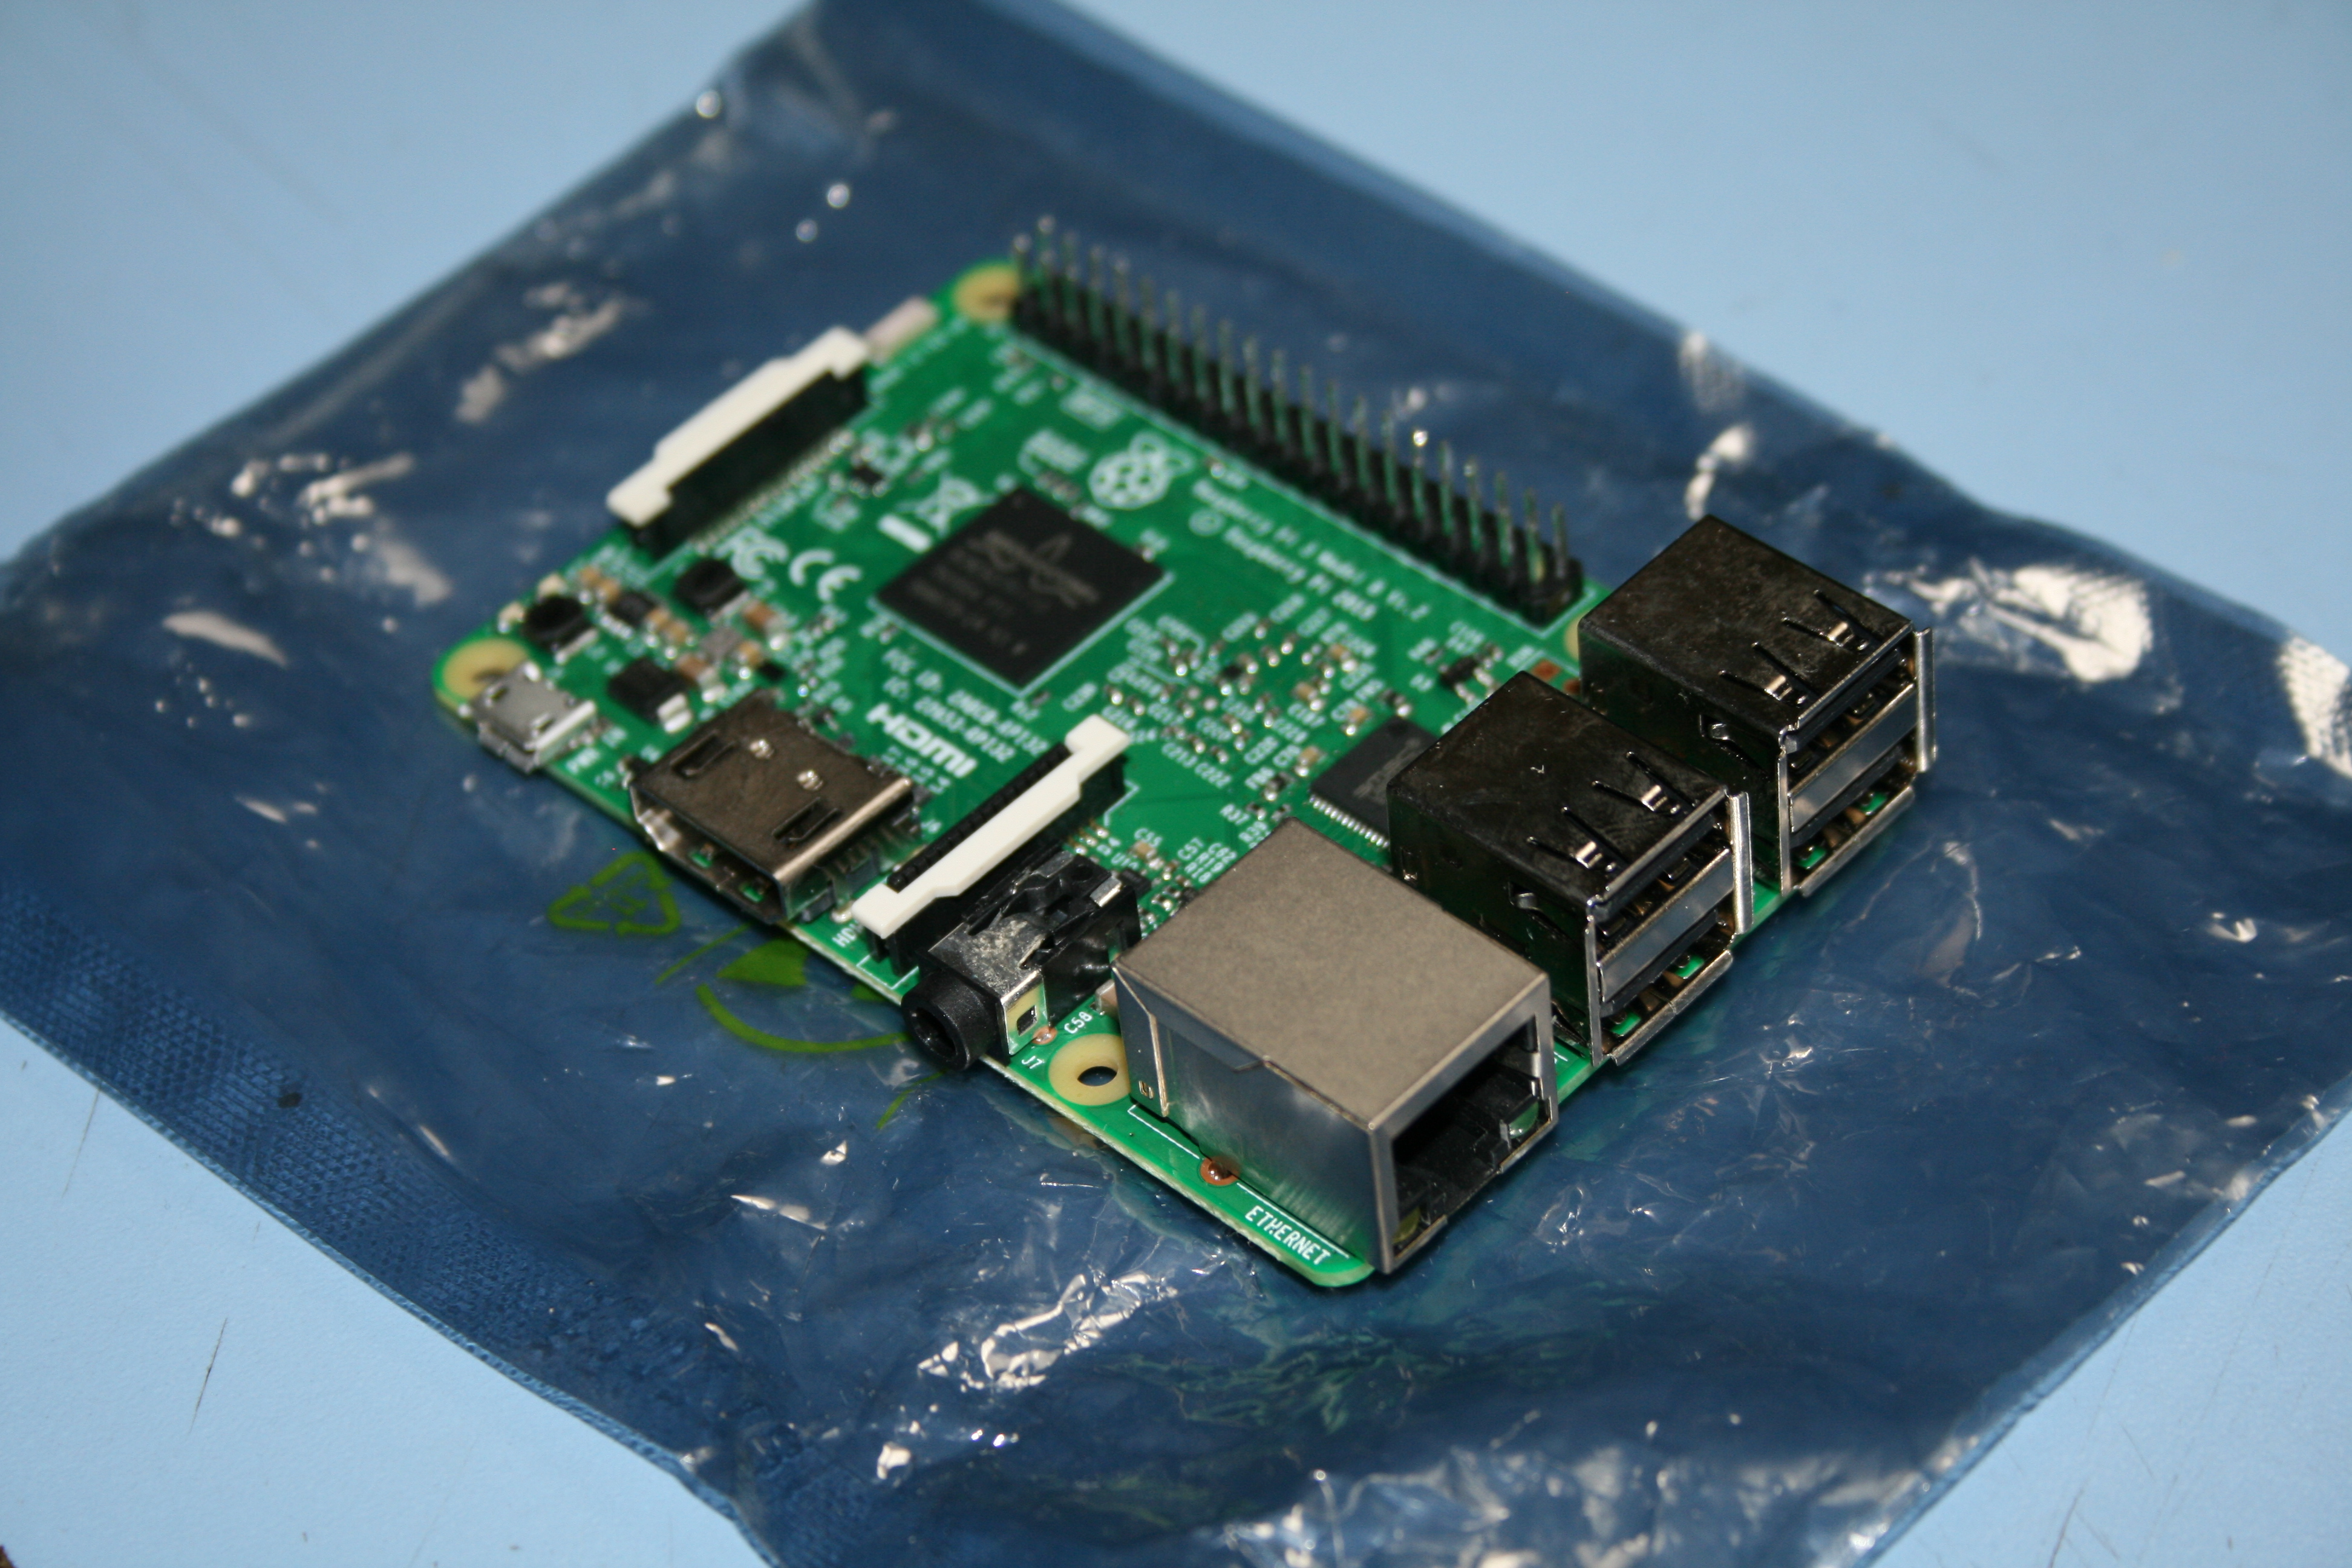
\includegraphics[width=.6\paperwidth]{images/rpi.jpg}}
\end{center}
		\caption{ \textit{Une Raspberry Pi}}
\end{figure}\\

La \textit{Raspberry Pi} est sans équivoque l'ordinateur du \textit{Maker} par excellence. Open source, elle permet de réaliser des systèmes embarqués performant pour un coût relativement faible et simple d'utilisation. Regardons ensemble les points du cahier des charges : 

\begin{enumerate}

\item Aucun pré-requis : Il s'agit ni plus ni moins que d'un ordinateur. J'ai détaillé cependant la façon dont on installe et configure l'OS pour la \textit{RaspberryPi}

\item Communication Ethernet : \textit{La Raspberry Pi}, comme tout bon ordinateur, possède une carte réseau et donc un port Ethernet. Noté toutefois, qu'à partir de la \textit{Raspberry Pi 3}, elle embarque également le \textit{Wi-Fi} et le \textit{Bluetooth}.

\item L'alimentation de la \textit{Raspberry Pi} se fait par un port micro-usb en \textit{5V}. La \textit{Raspberry Pi} ne gère pas l'alimentation \textit{PoE}. On peut alors recourir à une batterie ou bien à un \textit{PoE Splitter} qui récupère l'alimentation par le câble Ethernet et le transforme dans un port micro-usb.

\item Disposant d'une carte réseau, il n'y a aucun problème pour envoyer les données dans le cloud.

\item La \textit{Raspberry Pi} possède une sortie HDMI pour éventuellement brancher un écran. Il est également possible de mettre de petit écran LCD comme afficheur mais nous verrons ça plus tard.

\end{enumerate}

La \textit{Raspberry Pi} est alors un choix possible pour notre base de la station. Elle remplie effectivement toutes les conditions du cahier des charges.
\newpage
\subsection{\textit{L'Intel Edison}}

\textit{Intel} a décidé de se lancer dans l'IoT (il semblerait que le projet soit abandonnée) en sortant une puce : \textit{Edison}.
\begin{figure}[H]
\begin{center}
		\makebox[\textwidth]{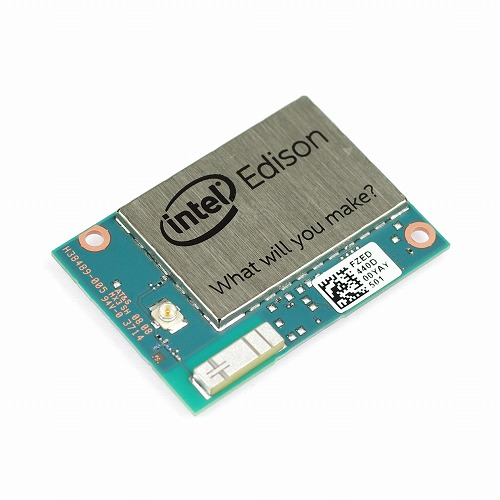
\includegraphics[width=.6\paperwidth]{images/edison.jpg}}
\end{center}
		\caption{ \textit{Une puce Edison}}
\end{figure}\\

Cette puce doit alors être placé sur une carte que fabrique également \textit{Intel} afin de pouvoir y brancher toute sorte de composants :\\

\begin{figure}[H]
\begin{center}
		\makebox[\textwidth]{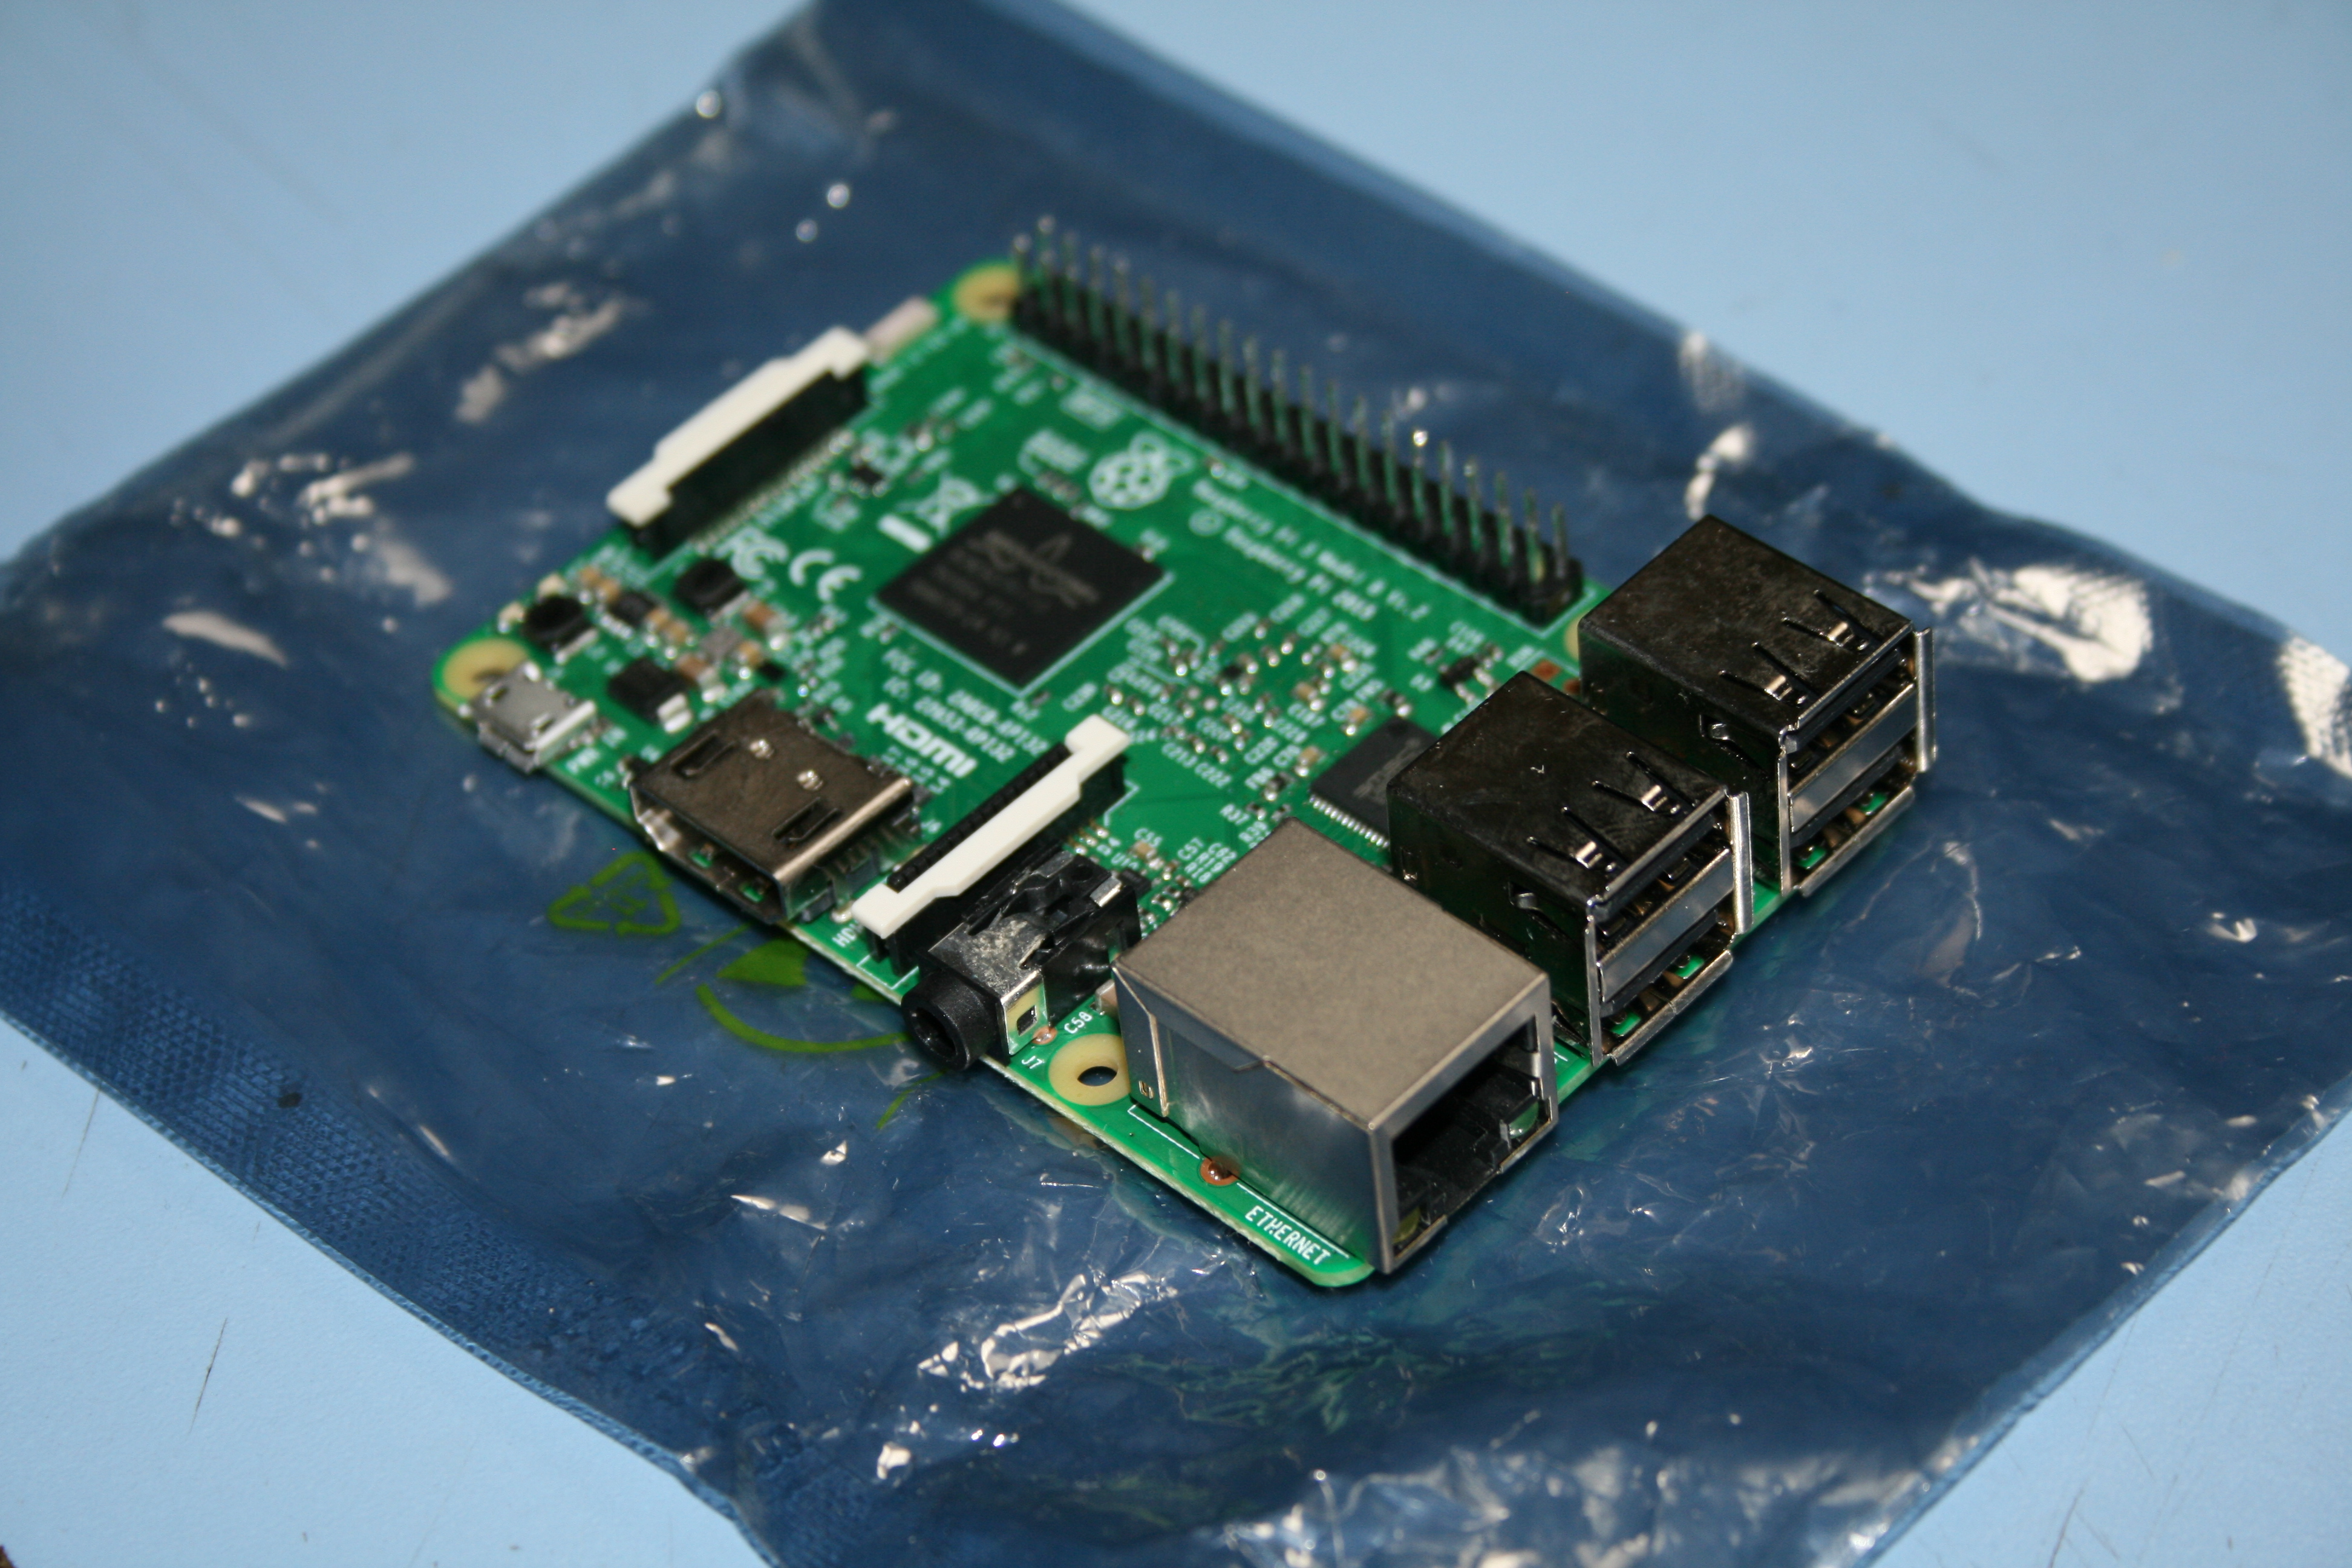
\includegraphics[width=.6\paperwidth]{images/rpi.jpg}}
\end{center}
		\caption{ \textit{Un intel Edison sur son board arduino}}
\end{figure}\\

Concrètement, il s'agit ni plus ni moins que d'un board Arduino amélioré. Amélioré par la performance de calcul de la puce \textit{Intel Edison} et amélioré car elle embarque un \textit{firmware} qui permet de compiler toute sorte de langage, dont le langage Arduino.\\

Le langage Arduino est parfait pour une mission comme la station car parfaitement adapté pour de l'électronique embarqué. Regardons les conditions du cahier des charges : 

\begin{enumerate}
\item Aucun pré-requis technique : De la même façon que pour la \textit{Raspberry Pi}, il suffit d'installer le \textit{firmware} dans une micro-SD par le biais d'un utilitaire très simple fournis par \textit{Intel}

\item L'intel ne dispose malheureusement pas ce carte réseau avec un port \textit{RJ45}. Il embarque cependant le \textit{Wi-Fi}. Comme ce dernier est embarqué sur un shield Arduino, on peut supposer qu'il est possible d'y installer un shield qui apporterais la fonctionnalité à notre système. Cela rendrait le système bien plus volumineux et complexe.

\item Ne possédant pas de port \textit{RJ45}, nous pouvons oublier la technologie \textit{PoE} sans l'utilisation d'un \textit{PoE Splitter} comme pour la \textit{Raspberry Pi}. L'alimentation pouvant se faire sur un micro-usb,il faudra donc opter pour la même solution.

\item Ayant la possibilité d'avoir un accès internet, il n'y aura donc aucun problème pour envoyer les données sur le \textit{Cloud Azure}. Il existe d'ailleurs de la documentation sur le site de \textit{Azure} concernant l'usage de \textit{L'intel Edison}.
\end{enumerate}

\textit{L'intel Edison} est donc un second choix possible même s'il est plus compliqué à mettre en place car nécessite plus de pièces.

\subsection{Le choix de la base de la station}

Comme je l'ai dit plus tôt, les deux choix sont possible. Il va alors falloir trancher au niveau du coût d'une part, puis de la simplicité de mise en place. Comme \textit{L'intel Edison} nécessite l'ajout d'un Shield pour pouvoir espérer un accès internet par câble, mon choix s'est porté sur la \textit{Raspberry Pi}.\\

\textit{L'intel Edison} se montre très intéressant de par sa puissance de calcul et ses possibilités, cependant, son coût est élevée et sa puissance se montre inutile pour l'usage que nous allons en avoir pour la station. Comme l'utilisation aurait été le même qu'un simple arduino uno, nous aurions pu envisager l'utilisation de ce dernier car il est un très bon choix en rapport qualité/prix. Il ne rivalise cependant pas en coût avec la \textit{Raspberry Pi}dès lors que nous ajoutons le shield Ethernet.\\

Ainsi, j'ai tout naturellement choisis la \textit{Raspberry Pi} pour réaliser la station. Il faut ensuite choisir les capteurs et autres composants que nous allons brancher à la \textit{Raspberry Pi}.

\section{Les composants}

Il faut maintenant faire une sélection de composants qui vont nous permettre de récolter les données, les afficher puis les envoyer dans le Cloud. Même si mon âme de roboticien voudrait créer une carte électronique où il suffirait de souder quelques composants pour avoir une plate forme faite sur mesure, il ne faut pas perdre de vu notre conditions "Aucun pré-requis". C'est pourquoi j'ai choisis d'utiliser les composants suivants : 

\subsection{Le Shield}

Pour réaliser une interface simpliste avec la \textit{Raspberry Pi} et les capteurs, nous allons utiliser un shield. Ce dernier porte le nom de \textit{GrovePi +}. 

\begin{figure}[H]
\begin{center}
	\makebox[\textwidth]{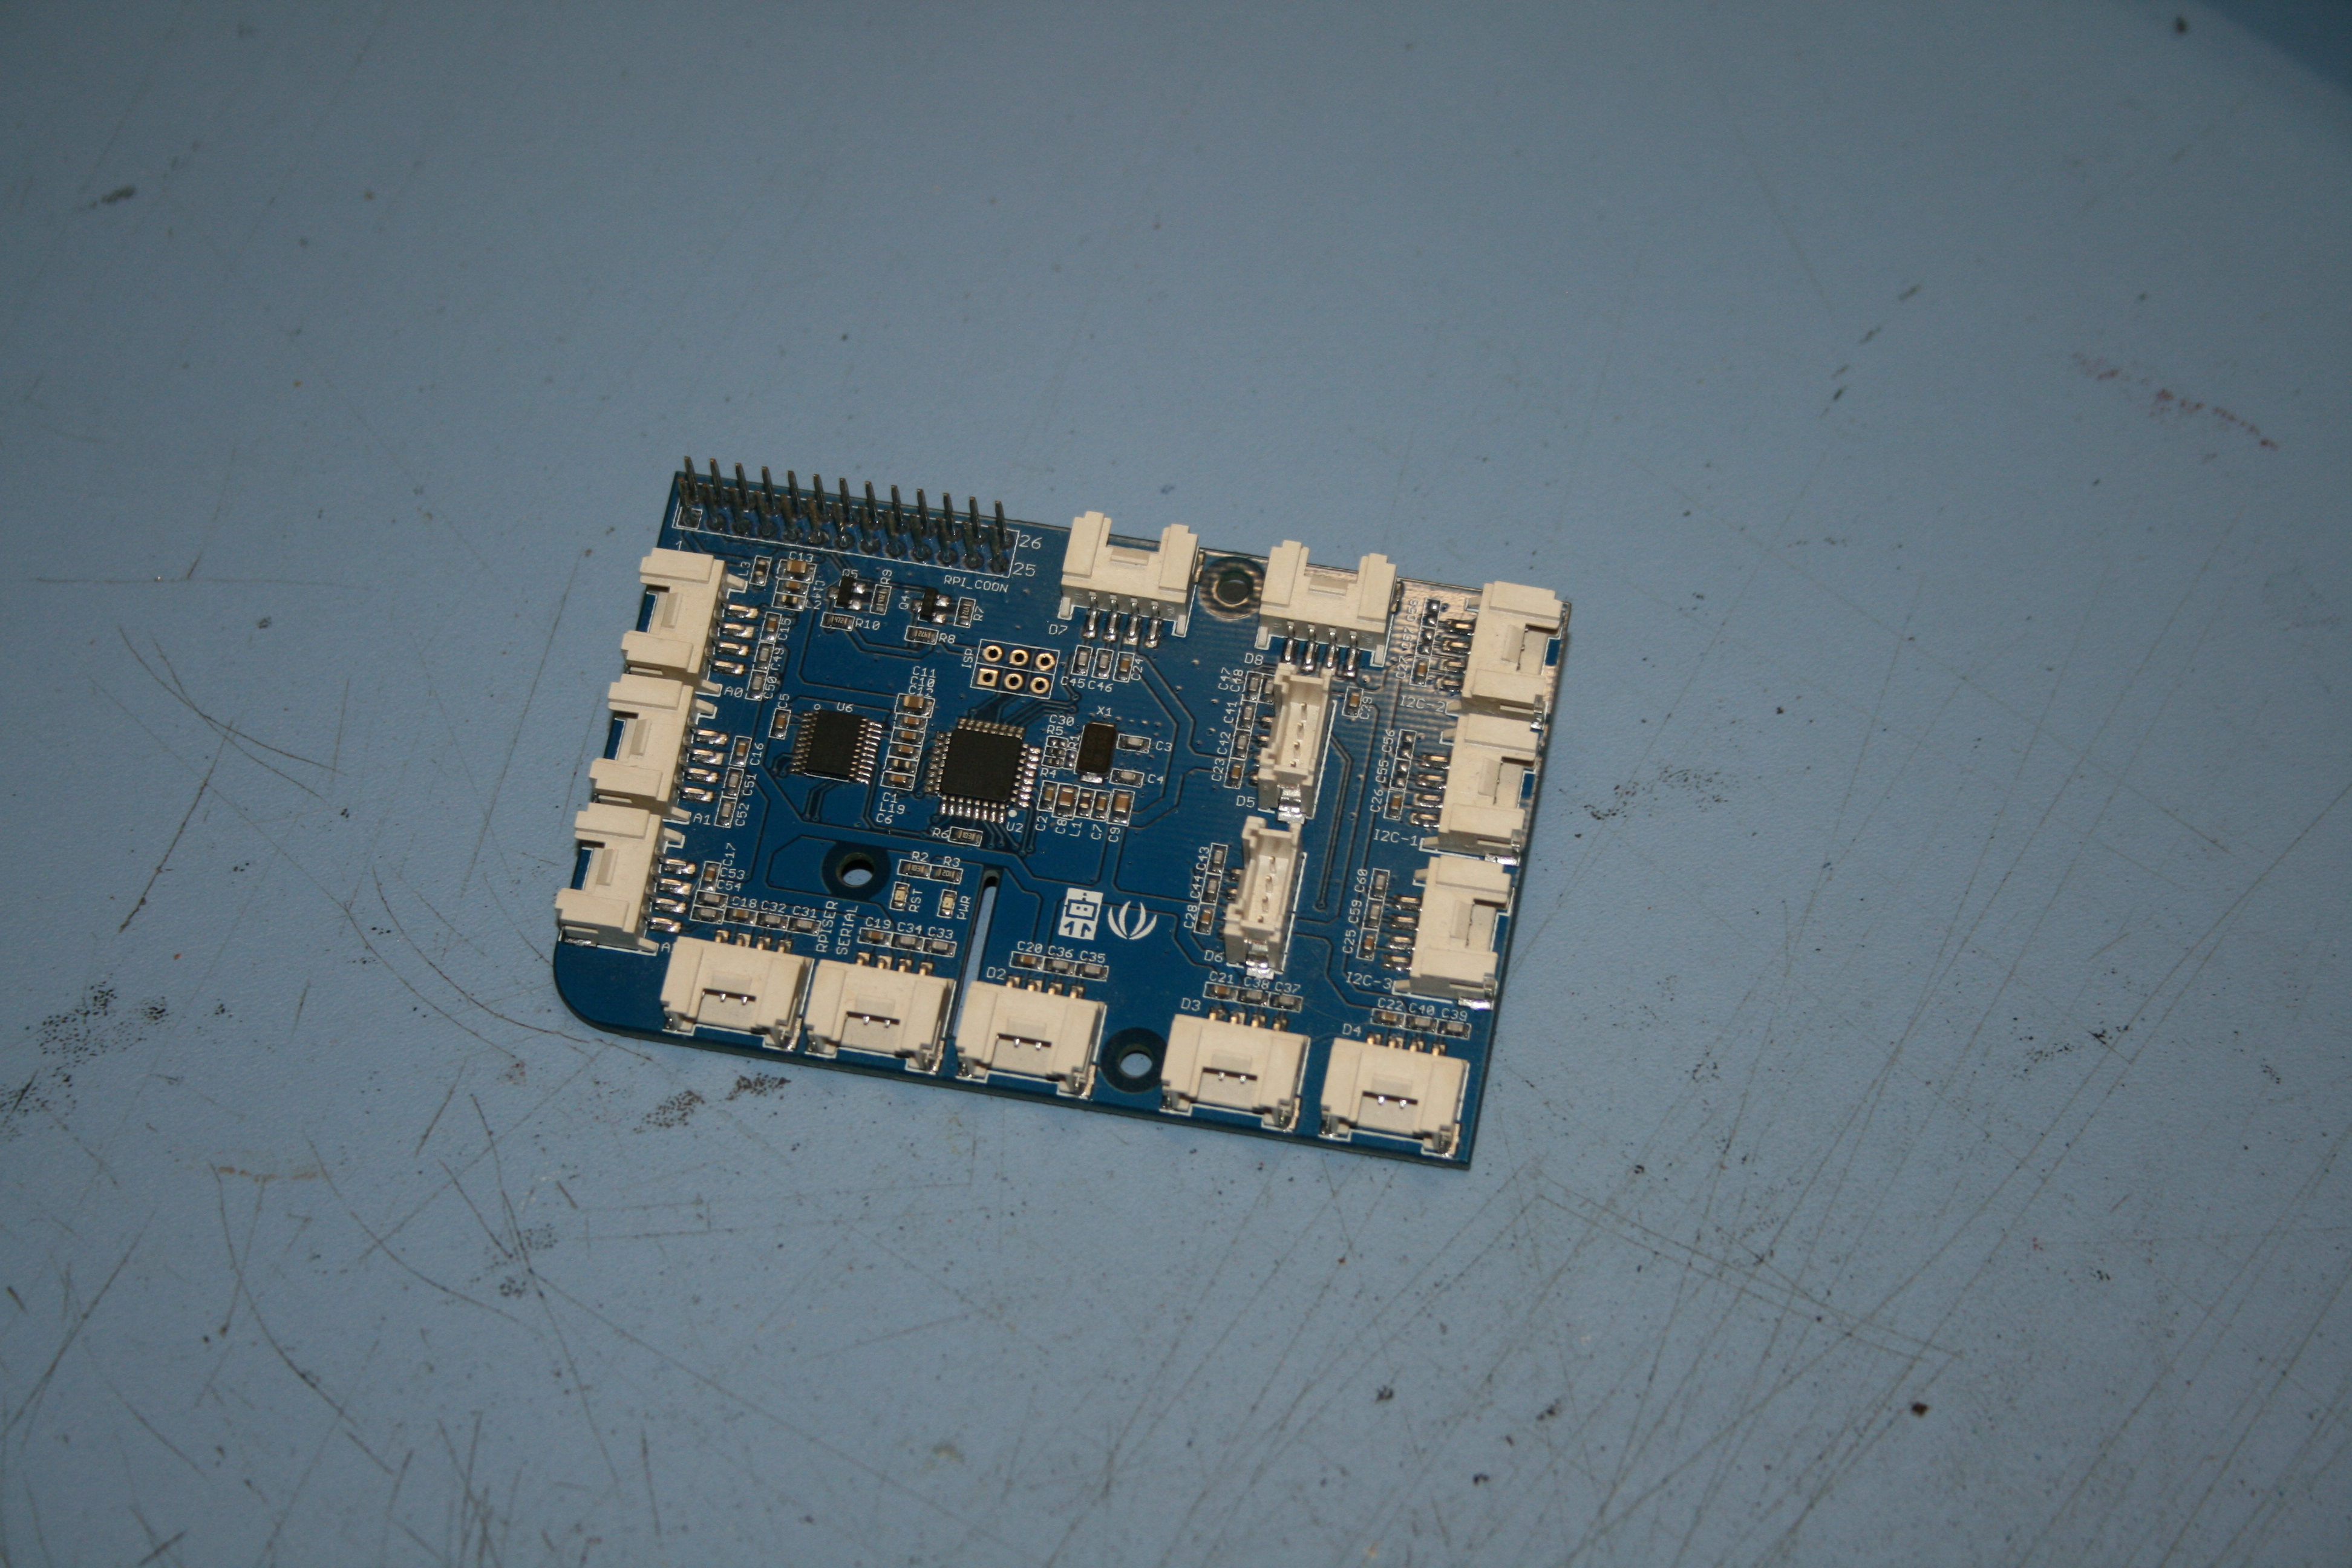
\includegraphics[width=.7\paperwidth]{images/grovepi.jpg}}
\end{center}
	\caption{ \textit{le Shield GrovePi+}}
\end{figure}\\

Pour \textit{l'Intel Edison} je parlais qu'il embarquait un board Arduino et compilais le langage Arduino (qui est ni plus ni moins qu'une version adapté de C++). Et bien ce shield est en réalité un Arduino qui communique avec la \textit{Raspberry Pi}. On notera le gros travail des ingénieurs qui ont réalisé les bibliothèques de tel sorte qu'il soit très facile de programmer pour l'utiliser mais nous détaillerons le langage de programmation dans une prochaine partie. Le seul bémol de ce Shield, c'est ses connecteurs 4-pin par lequel on branche les composants.\\

En effet, même s'il est simple et ludique de faire les branchements, cela oblige à acheter les composants qui sont déjà fabriqué pour être branché dessus. Du moins si l'on veut pas faire de soudure. Il serait possible de commander uniquement les connecteurs pour utiliser les composants que l'on souhaite mais ce n'est pas l'objectif ici.\\

\subsection{Capteur de température et d'humidité}

Le capteur que j'ai choisi ici est le DHT22.\\

Après plusieurs test avec son petit frère, le DHT11, j'ai décidé qu'il serait plus judicieux de monter en gamme car ce dernier manquait cruellement de précision. Ce genre de capteur sont cependant pas fait pour avoir une température instantanée. En effet, leur conception font qu'ils sont relativement lent pour réagir aux choc de température. Ces capteurs sont en effet là pour avoir une courbe de tendance de la température. Nous allons avoir l'allure de la variation de la température sur de longue durée de l'ordre de plusieurs heure. C'est pour ça qu'il n'est pas impossible de voir quelques valeurs faussée à quelques instants.\\

\subsection{Capteur de luminosité}

Les capteurs de luminosité sont très imprécis car la mesure de la luminosité avec précision coûte très chère. Cependant, nous n'avons pas besoin de mesurer de façon exacte la luminosité. D'une part car son unité, le luxmètre n'est pas très parlant pour le grand public et d'autre part, nous voulons juste avoir une information nous permettant de définir si la lumière d'une pièce serait allumée ou éteinte.\\

J'ai donc testé le capteur en le laissant tourner durant 2 jours complets pour voir un seuil à partir duquel on pouvait définir que la lumière était effectivement éteinte.\\

A noter cependant que ce seuil a été choisi arbitrairement et qu'il pourrait ne pas fonctionner selon les endroit où est placé la station (au bord d'une fenêtre typiquement).\\


\subsection{L'écran d'affichage}

Comme je l'ai spécifié dans le cahier des charges, il fallait pouvoir récupérer les valeurs localement. J'ai donc installé un écran afficheur 2x16 caractères.
De cette façon, la station pourra afficher les valeurs.\\

\subsection{L'encodeur rotatif}

L'écran ayant une capacité d'affichage limitée, j'ai ajouté un encodeur rotatif pour naviguer entre différents menu sur l'écran pour afficher différentes valeurs utile.\\

\subsection{PoE Splitter}

Le PoE Splitter va permettre d'alimenter la \textit{RaspberryPi} en PoE en découpant le câble RJ45 en 2 canaux : Un sur un câble micro - USB pour l'alimentation et un câble Ethernet RJ45 pour relier la station au réseau.

\section{Le langage de programmation}

Avec le \textit{Shield}, il était possible d'utiliser une multitude de langage de programmation. Cependant il fallait un langage intuitif et simple car il y a des lignes qui devront être changé lors d'un déploiement comme le nom des ressources sur Microsoft Azure où envoyer les données. J'ai automatiquement pensé au langage Python. Il est le langage de haut niveau par excellence. De plus, il est relativement adapté pour des script embarqué. Il n'est pas rare de voir des code de pilotage de robot fait en Python.

Voici un petit aperçu du code : 

\newpage
\pythonexternal{./station.py}\\

\section{Le coût d'une station}

Regroupons dans un premier temps le coût matériel, puis nous discuterons ensuite du coût logiciel, notamment sur \textit{Azure}.\\

\subsection{Coût du matériel}

Je vous propose donc le tableau ci-dessous réalisant l'inventaire des pièces nécessaire ainsi que de leur coût moyen en me basant sur deux sites : \textit{Amazon} et \textit{Seeed Studio}, qui est le distributeur de GrovePi+. Attention par contre à vérifier les provenance de Seeed car je me demande s'il n'est pas possible que des frais de douanes s'appliquent sur leur produits.

\begin{center}

	\begin{tabular}{|l|l|l|l|}
		\hline
		Composant & Prix & Amazon & Seeed \tabularnewline
		\hline
		RaspberryPi 3 & 35 euros & \href{ https://www.amazon.fr/Raspberry-Pi-Carte-M%C3%A8re-Model/dp/B01CD5VC92/ref=sr_1_3?s=computers&ie=UTF8&qid=1501236508&sr=1-3&keywords=raspberry+pi+3}{Amazon} & \href{https://www.seeedstudio.com/Raspberry%20Pi%203%20Model%20B-p-2625.html}{Seeed}\tabularnewline
		\hline
		Shield GrovePi+ & 33 euros & \href{https://www.amazon.fr/SEEEDSTUDIO-Seeedstudio-grovepi/dp/B01AFKN2TK/ref=sr_1_1?ie=UTF8&qid=1501238966&sr=8-1&keywords=grovepi%2B}{Amazon} & \href{https://www.seeedstudio.com/GrovePi%2B-p-2241.html}{Seeed}\tabularnewline
		\hline
		DHT22 & 17 euros & \href{https://www.amazon.fr/Accuracy-Temperature-Humidity-Raspberry-Platforms/dp/B01FY5EBO6/ref=sr_1_cc_1?s=aps&ie=UTF8&qid=1501239845&sr=1-1-catcorr&keywords=Temperature%26Humidity+Sensor+Pro}{Amazon} & \href{https://www.seeedstudio.com/Grove-Temperature%26Humidity-Sensor-Pro-p-838.html}{Seeed}\tabularnewline
		\hline
		Luminosite & 3 euros & & \href{https://www.seeedstudio.com/Grove-Light-Sensor-p-746.html}{Seeed}\tabularnewline
		\hline
		Ecran & 16 euros & \href{https://www.amazon.fr/gp/offer-listing/B01AFKPJ6O/ref=dp_olp_0?ie=UTF8&condition=all&qid=1501240259&sr=8-1}{Amazon} & \href{https://www.seeedstudio.com/Grove-LCD-RGB-Backlight-p-1643.html}{Seeed}\tabularnewline
		\hline
		Bouton rotatif & 5 euros & \href{https://www.amazon.fr/Seeedstudio-Grove-Capteur-Rotary-Angle-P/dp/B01AFKNFJM/ref=sr_1_fkmr0_3?ie=UTF8&qid=1501240488&sr=8-3-fkmr0&keywords=Grove+-+Rotary+Angle+Sensor%28P%29}{Amazon} & \href{https://www.seeedstudio.com/Grove-Rotary-Angle-Sensor%28P%29-p-1242.html}{Seeed}\tabularnewline
		\hline
		PoE Spliter & 10 euros & \href{https://www.amazon.fr/DSLRKIT-Active-Splitter-Ethernet-Raspberry/dp/B01H37XQP8/ref=sr_1_2?s=computers&ie=UTF8&qid=1501240606&sr=1-2&keywords=poe+splitter}{Amazon} &\tabularnewline
		\hline
		Micro SG (8Gb min) & 8 euros & & \tabularnewline
		\hline
		Total & 127 euros & &\tabularnewline
		\hline
	\end{tabular}
\end{center}\\

Nous avons donc un coût total moyen de l'ordre de 130€ par station. A noter qu'il s'agit d'un prix à l'unité, les commandes en gros jouissant de réduction sur Seeed Studio.\\

De plus, compter 2 à 3 euros de matière plastique si vous voulez imprimer un bouton et une coque (on ne rentrera pas l'imprimante 3D dans le coût).\\

\subsection{Coût logiciel}

Côté logiciel, j'ai utilisé un OS \textit{OpenSource} et crée le code pour le bon fonctionnement de la station. Les logiciels tiers pour la configuration sont entièrement gratuit.\\

Le seul coût vient alors sur le Cloud \textit{Azure}.\\

Mes estimations sont à revoir avec un conseiller chez \textit{Microsoft Azure} car je ne suis pas certain.\\

J'estime le tarif à minimum 1






